\section{Une épidémie (7 points)}

Une épidémie affecte une île du Pacifique, depuis le mois d'avril 2013. Nous disposons des données du nombre de personnes infectées sur les mois d'avril à septembre 2013. Ces données sont récapitulées dans le tableau suivant :

\vspace*{0.5cm} 
\begin{center}
	\begin{tabular}{|@{\ }l@{\ }|@{\ }c@{\ }|@{\ }c@{\ }|@{\ }c@{\ }|@{\ }c@{\ }|@{\ }c@{\ }|@{\ }c@{\ }|}
		\hline
		Mois                                & Avril      & Mai        & Juin & Juillet    & Août & Septembre \\ \hline
		Rang du mois $x_i$                  & 0          & 1          & 2    & 3          & 4    & 5         \\ \hline
		Nombre de malades en milliers $y_i$ & \num{17.5} & \num{27.5} & 35   & \num{42.5} & 49   & 51        \\ \hline
	\end{tabular}
\end{center}

\begin{questions}
	\question[1] En observant le nuage de points correspondant au tableau, tracé ci-dessous, un ajustement affine est-il envisageable ?
	\begin{solution}
		Oui, un ajustement affine est envisageable car le nuage de point est allongé.
	\end{solution}
	
	\question[1\half] Calculer les coordonnées du point moyen $G$ du nuage de points et l'ajouter sur le nuage de points.
	\begin{solution}
		Calcul des coordonnées du point moyen G :
		
		\begin{eqnarray*}
			\bar{X} &=& \frac{0 + 1 + 2 + 3 + 4 + 5 }{6}\\
			\bar{X} &=& \frac{14}{6}\\
			\bar{X} &=& \num{2.5}
		\end{eqnarray*}
	
		\begin{eqnarray*}
			\bar{Y} &=& \frac{\num{17.5} + \num{27.5} + 35 + \num{42.5} + 49 + 51 }{6}\\
			\bar{Y} &=& \frac{\num{222.5}}{6}\\
			\bar{Y} &\approx& 31			
		\end{eqnarray*}
	
		Donc les coordonnées du point G sont $(\num{2.5}; 31)$.
	\end{solution}
	
	\question[2] On considère la droite $(d)$, d'équation $y = \num{6.8} x + 20$, réalise un bon ajustement du nuage de points. Tracer la droite $(d)$.
	
	\question En utilisant l'approximation affine précédente, déterminer par le calcul :
	\begin{parts}
		\part[1\half] le nombre de personnes atteintes en février 2014 ;
		
		\begin{solution}
			Le mois 0 est avril 2013, il y a 10 mois entre avril 2013 et février 2014. Je cherche le nombre de malades pour le mois de rang 10  :
			
			\begin{eqnarray*}
				y &=& \num{6.8} x + 20 \\
				y &=& \num{6.8} \times 10 - 20\\
				y &=& 68 + 20 \\
				y &=& 88
			\end{eqnarray*}
			
			En février 2014 il y aura \num{88000} personnes atteintes.
		\end{solution}
		\part[1\half] le mois à partir duquel la population atteinte dépassera \num{10000} personnes.
		\begin{solution}
			Je cherche le rang du mois où on dépassera les  \num{10000} malades :
			
			\begin{eqnarray*}
				y &=& \num{6.8} x + 20 \\
				100 &\leq& \num{6.8} \times x + 20\\
				100 - 20 &\leq& \num{6.8} \times x \\
				80 &\leq& \num{6.8} \times x \\
				\frac{80}{\num{6.8}} &\leq& x \\
				\num{11.7} &\leq& x
			\end{eqnarray*}
			
			Il faudra attendre plus de 11 mois pour dépasser les \num{100000} personnes atteintes, soit avril 2014.
		\end{solution}
	\end{parts}
	
\end{questions}

\begin{center}
	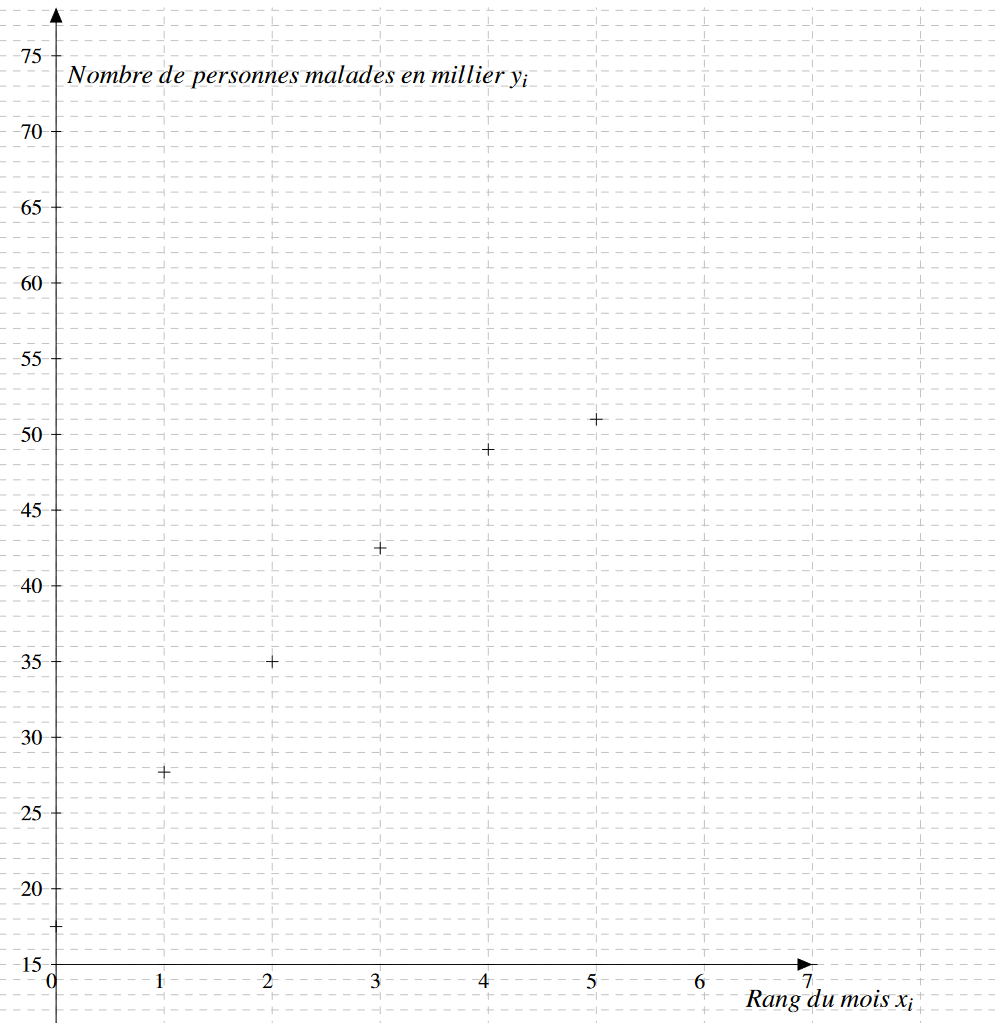
\includegraphics[scale=0.5]{nuage}
\end{center}